\section{Results}

When discussing results, I refer to conditions with acronyms NM for Nelder-Mead, and BO for Bayesian optimization.

First, which algorithm was better able to help participants achieve their goals?
In the BO condition, participants' best-rated configurations were much closer to their goal than in the NM condition (see Figure~\ref{fig:bestfits}),
By looking at longitudinal data (Figure~\ref{fig:best_distances}), it appears that by iteration 10, participants in the BO condition were, in general, closer to their goal than participants in the NM condition.

\begin{figure}
  \centering
  \begin{subfigure}[b]{0.23\textwidth}
    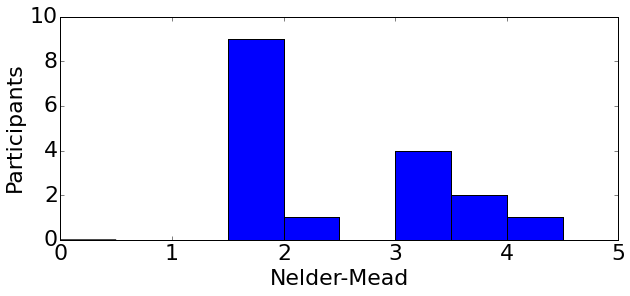
\includegraphics[width=\textwidth]{figures/bestfits_nm}
  \end{subfigure}
  \begin{subfigure}[b]{0.23\textwidth}
    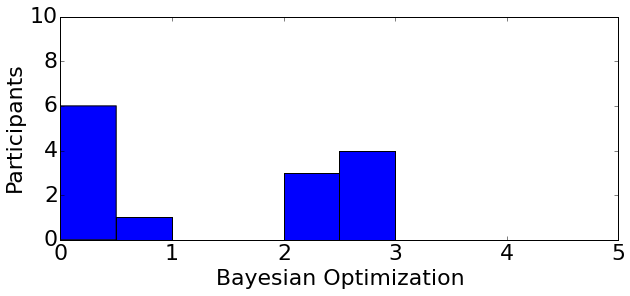
\includegraphics[width=\textwidth]{figures/bestfits_bo}
  \end{subfigure}
  \caption{Best fits for Nelder-Mead}\label{fig:bestfits}
\end{figure}

\begin{figure}
\centering
  \begin{subfigure}[b]{0.48\textwidth}
    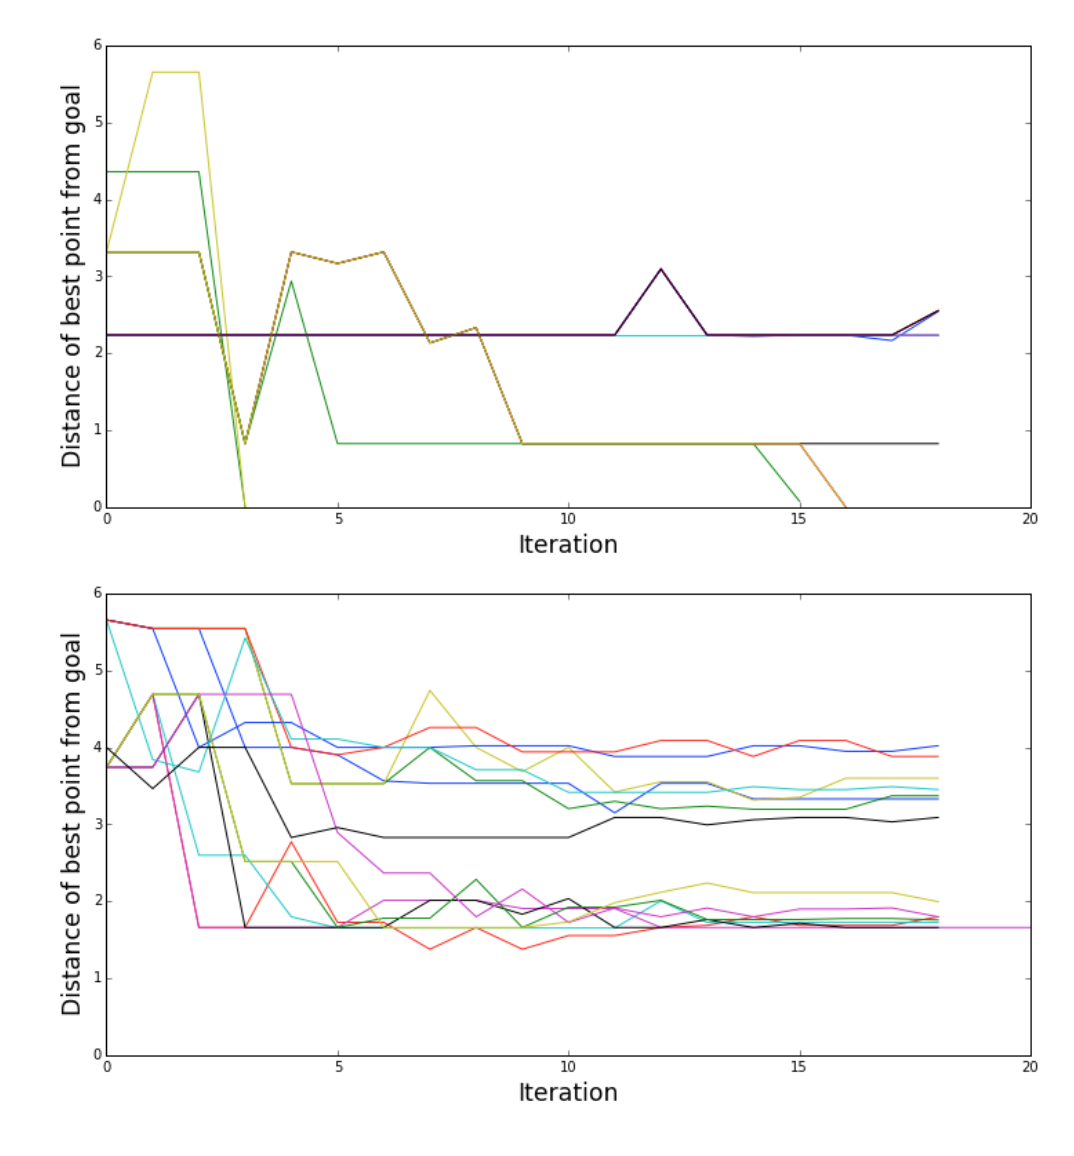
\includegraphics[width=\textwidth]{figures/best_distances}
    \caption{%
      With each successive ranking, the distance of a participant's best-rated point from the goal configuration.
    }\label{fig:best_distances}
  \end{subfigure}
  \begin{subfigure}[b]{0.48\textwidth}
    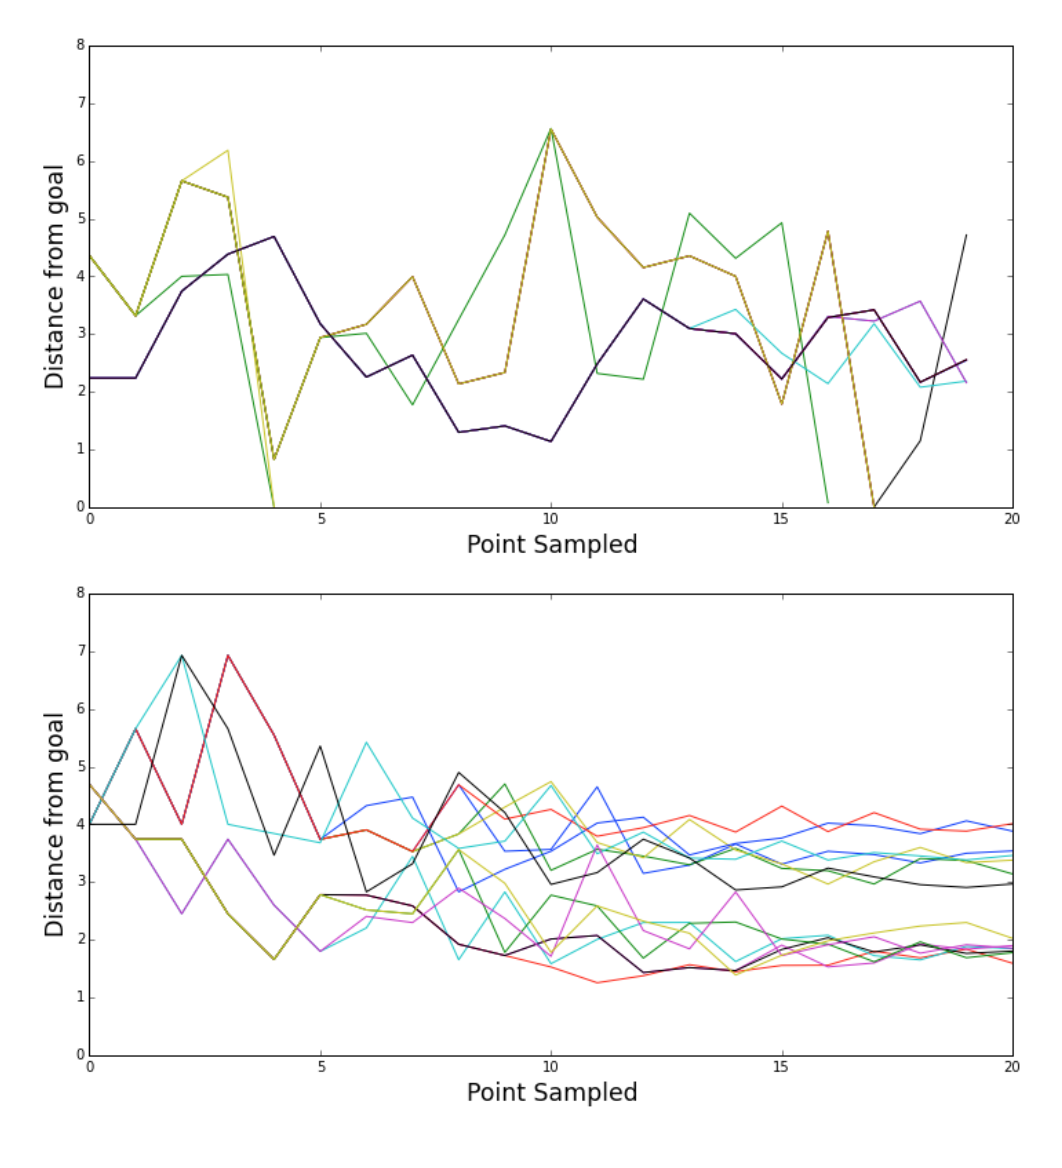
\includegraphics[width=\textwidth]{figures/point_distances}
    \caption{%
      The distance of each new point an algorithm proposes from the goal configuration.
    }\label{fig:point_distances}
  \end{subfigure}
  \caption{%
    Distances of best-rated or proposed points from goal configurations.
    Each line represents one participant working with one algorithm.
    For each pair of plots ((a) and (b)),
    Bayesian optimization is shown on the top, and 
    Nelder-Mead is shown on the bottom.
  }
\end{figure}

When we observe the paths of points provided by each of the algorithms, we see differing approaches in the points proposed.
In its current form, participants using BO clearly covered more of the parameter space (see Figure~\ref{fig:coverage}).
For NM, it appears that vertices were gradually pulled in toward the some center where the simplex converged.
In fact, this motion looks mostly planar.
BO, in comparison, appears almost like random sampling.
This may be in part due to our particular choice of kernel $\sigma$ and noise standard deviation $\sigma_{noise}$.

\begin{figure}
  \centering
  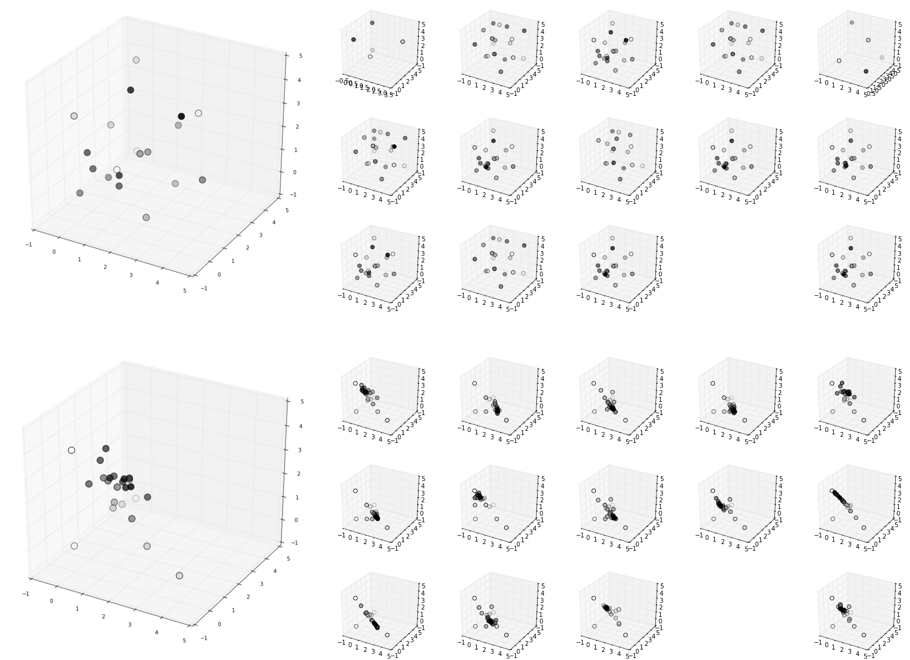
\includegraphics[width=0.48\textwidth]{figures/scatters}
  \caption{%
    The points that each algorithm proposed.
    The first three rows show participants using Bayesian optimization.
    The bottom three rows show participants using Nelder-Mead.
    An enlarged exemplar for each method is shown to the left of the small multiples.
    The first point an algorithm proposes is shown in white;
    Each new point is more grey than the last, until the final point is black.
  }\label{fig:coverage}
\end{figure}

When we consider the distance of each of the proposed points from the goal, we see why BO outperformed NM\@.
Figure~\ref{fig:point_distances} shows how the distance of the latest point proposed changes over time for each algorithm.
After about the tenth point sampled, it appears as if Nelder-Mead no longer suggests new examples radically farther from the goal.
This may be an indication of NM prematurely converging to a local maximum.
BO, on the other hand, continues to suggest points both near and far from the goal, and does not appear to converge at all.

Participants perceived these differences in how the algorithms worked (see Figure~\ref{fig:feedback}).
Those in the BO condition were more likely to report that the algorithm's choice of points seemed random.
But these participants were also more likely to claim that the point they marked as the best was very close to the goal.
Participants working with NM more often reported that the algorithm seemed to improve over time.
However, it also seemed more likely to get stuck.

\begin{figure}
  \centering
  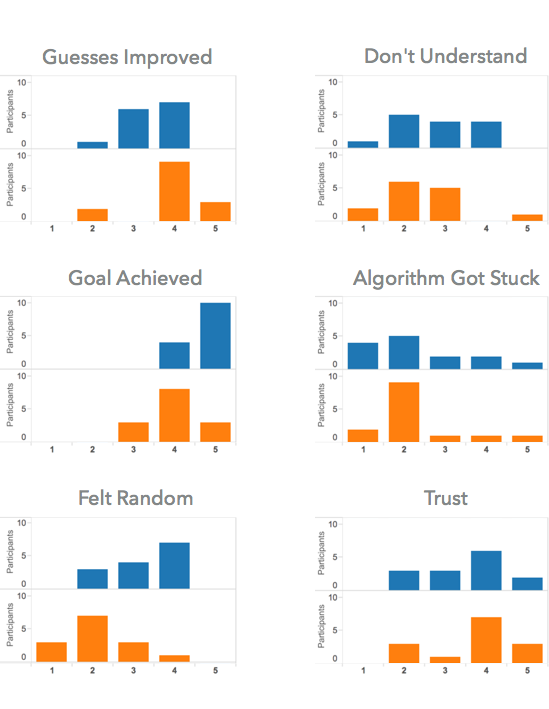
\includegraphics[width=0.4\textwidth]{figures/feedback}
  \caption{%
    Participant responses to questions about their perception of each algorithm.
    Blue bars show participants in the Bayesian optimization condition.
    Orange bars show participants in the Nelder-Mead condition.
  }\label{fig:feedback}
\end{figure}

\subsection{Limitations}

Participants were forced to stop after reporting 20 rankings to the algorithm.
I expect that that the Bayesian optimization algorithm would have seemed less random over time.
The choice of hyperparameters for NM and BO might impact user perceptions of randomness and the best point a participant finds after 20 rankings.
Before drawing any conclusions about these algorithms, a wider, systematically-determined range of hyperparameters must be tested.

Many of the participants in the BO condition achieved exactly the goal after only a few rankings (see Figure~\ref{fig:coverage}).
It's likely that one of the goals was ``just right'' for participants in the BO condition to discover precisely the right condition after only a few comparisons.
This suggests that this one goal was better suited to BO than NM for these tests, and weakens any potential claims about inherent strengths of BO at finding configurations close to the goal.
To counter this side effect and improve generalizability, a larger number of goal images should be tested.
Better yet, goal images could be randomly selected from the domain of the input space.
